\documentclass{standalone}
\usepackage{tikz}
\usetikzlibrary{patterns, positioning}

\begin{document}
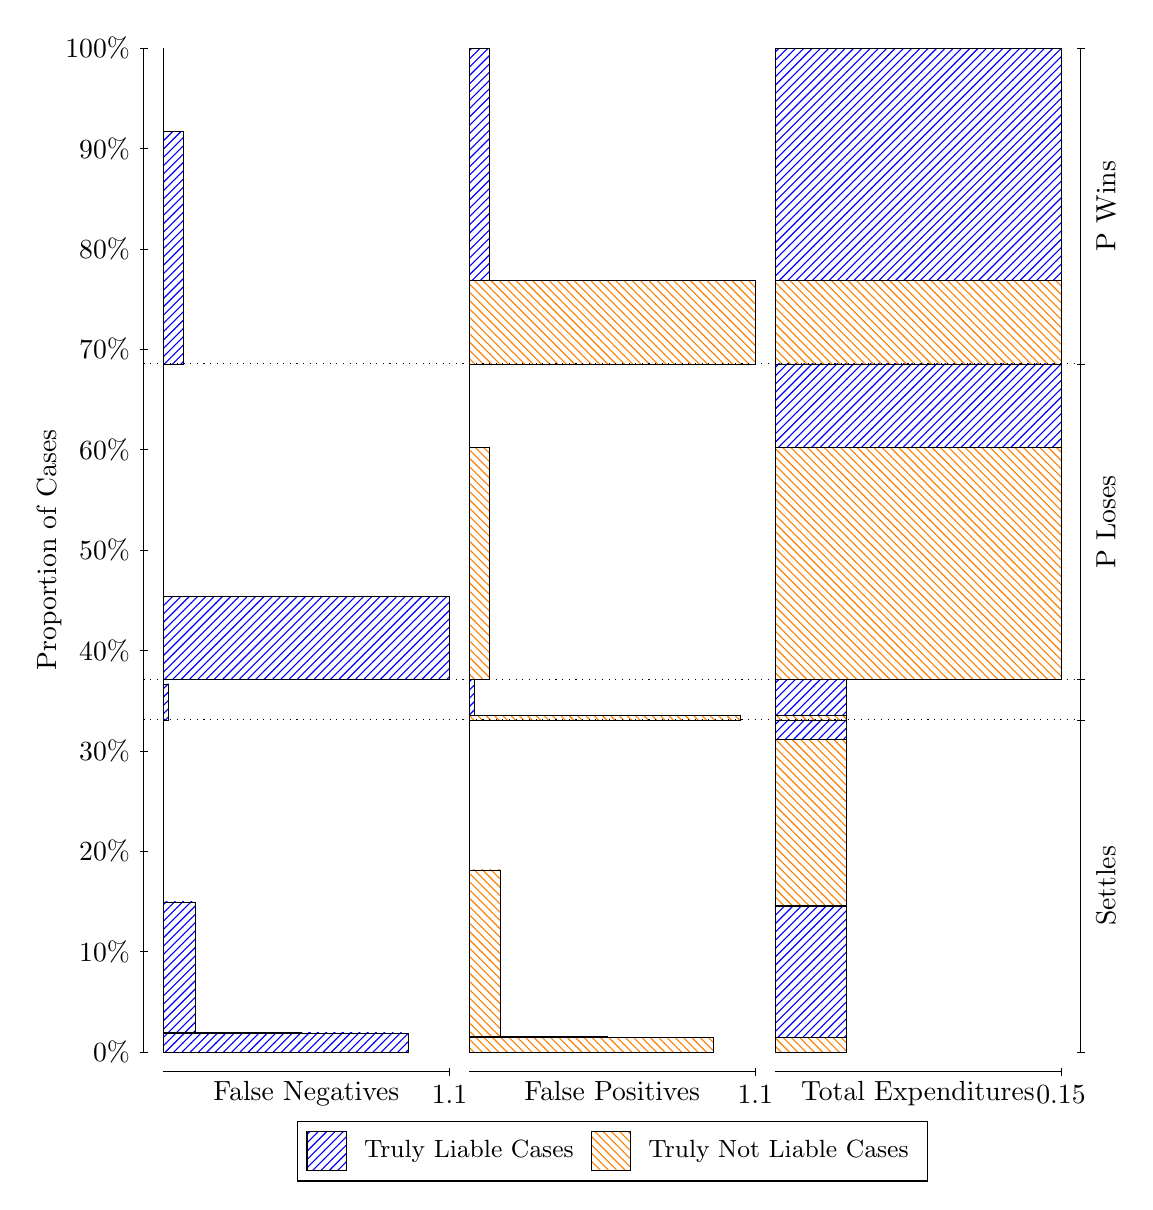
\begin{tikzpicture}
\draw[black, very thin] (1.5,1.75) -- (1.5,14.5);
\node[rotate=90, anchor=center] at (0.3, 8.125) {Proportion of Cases};
\draw[black, very thin] (1.45,1.75) -- (1.55,1.75);
\node[anchor=east] at (1.45, 1.75) {0\%};
\draw[black, very thin] (1.45,3.025) -- (1.55,3.025);
\node[anchor=east] at (1.45, 3.025) {10\%};
\draw[black, very thin] (1.45,4.3) -- (1.55,4.3);
\node[anchor=east] at (1.45, 4.3) {20\%};
\draw[black, very thin] (1.45,5.575) -- (1.55,5.575);
\node[anchor=east] at (1.45, 5.575) {30\%};
\draw[black, very thin] (1.45,6.85) -- (1.55,6.85);
\node[anchor=east] at (1.45, 6.85) {40\%};
\draw[black, very thin] (1.45,8.125) -- (1.55,8.125);
\node[anchor=east] at (1.45, 8.125) {50\%};
\draw[black, very thin] (1.45,9.4) -- (1.55,9.4);
\node[anchor=east] at (1.45, 9.4) {60\%};
\draw[black, very thin] (1.45,10.675) -- (1.55,10.675);
\node[anchor=east] at (1.45, 10.675) {70\%};
\draw[black, very thin] (1.45,11.95) -- (1.55,11.95);
\node[anchor=east] at (1.45, 11.95) {80\%};
\draw[black, very thin] (1.45,13.225) -- (1.55,13.225);
\node[anchor=east] at (1.45, 13.225) {90\%};
\draw[black, very thin] (1.45,14.5) -- (1.55,14.5);
\node[anchor=east] at (1.45, 14.5) {100\%};

\draw[black, very thin] (13.4,1.75) -- (13.4,14.5);
\draw[black, very thin] (13.35,1.75) -- (13.45,1.75);
\node[anchor=west] at (13.35, 1.75) {};
\draw[black, very thin] (13.35,5.9689) -- (13.45,5.9689);
\node[anchor=west] at (13.35, 5.9689) {};
\draw[black, very thin] (13.35,6.4775) -- (13.45,6.4775);
\node[anchor=west] at (13.35, 6.4775) {};
\draw[black, very thin] (13.35,10.489) -- (13.45,10.489);
\node[anchor=west] at (13.35, 10.489) {};
\draw[black, very thin] (13.35,14.5) -- (13.45,14.5);
\node[anchor=west] at (13.35, 14.5) {};

\draw[black, very thin, pattern color=blue, pattern=north east lines] (1.75,1.75) rectangle (4.8552,1.9914);
\draw[black, very thin, pattern color=blue, pattern=north east lines] (1.75,1.9914) rectangle (4.5172,1.9919);
\draw[black, very thin, pattern color=blue, pattern=north east lines] (1.75,1.9919) rectangle (4.1793,1.9924);
\draw[black, very thin, pattern color=blue, pattern=north east lines] (1.75,1.9924) rectangle (3.8413,1.9929);
\draw[black, very thin, pattern color=blue, pattern=north east lines] (1.75,1.9929) rectangle (3.5033,1.9996);
\draw[black, very thin, pattern color=blue, pattern=north east lines] (1.75,1.9996) rectangle (2.1514,3.6571);
\draw[black, very thin, pattern color=orange, pattern=north west lines] (1.75,3.6571) rectangle (1.75,5.9689);
\draw[black, very thin, pattern color=blue, pattern=north east lines] (1.75,5.9689) rectangle (1.8134,6.4254);
\draw[black, very thin, pattern color=orange, pattern=north west lines] (1.75,6.4254) rectangle (1.75,6.4775);
\draw[black, very thin, pattern color=blue, pattern=north east lines] (1.75,6.4775) rectangle (5.3833,7.5408);
\draw[black, very thin, pattern color=orange, pattern=north west lines] (1.75,7.5408) rectangle (1.75,10.489);
\draw[black, very thin, pattern color=blue, pattern=north east lines] (1.75,10.489) rectangle (2.0035,13.437);
\draw[black, very thin, pattern color=orange, pattern=north west lines] (1.75,13.437) rectangle (1.75,14.5);
\draw[black, very thin, pattern color=orange, pattern=north west lines] (5.6333,1.75) rectangle (8.7386,1.939);
\draw[black, very thin, pattern color=orange, pattern=north west lines] (5.6333,1.939) rectangle (7.3866,1.9457);
\draw[black, very thin, pattern color=orange, pattern=north west lines] (5.6333,1.9457) rectangle (7.0486,1.9462);
\draw[black, very thin, pattern color=orange, pattern=north west lines] (5.6333,1.9462) rectangle (6.7107,1.9467);
\draw[black, very thin, pattern color=orange, pattern=north west lines] (5.6333,1.9467) rectangle (6.3727,1.9471);
\draw[black, very thin, pattern color=orange, pattern=north west lines] (5.6333,1.9471) rectangle (6.0347,4.0618);
\draw[black, very thin, pattern color=blue, pattern=north east lines] (5.6333,4.0618) rectangle (5.6333,5.9689);
\draw[black, very thin, pattern color=orange, pattern=north west lines] (5.6333,5.9689) rectangle (9.0766,6.0209);
\draw[black, very thin, pattern color=blue, pattern=north east lines] (5.6333,6.0209) rectangle (5.6967,6.4775);
\draw[black, very thin, pattern color=orange, pattern=north west lines] (5.6333,6.4775) rectangle (5.8868,9.4255);
\draw[black, very thin, pattern color=blue, pattern=north east lines] (5.6333,9.4255) rectangle (5.6333,10.489);
\draw[black, very thin, pattern color=orange, pattern=north west lines] (5.6333,10.489) rectangle (9.2667,11.552);
\draw[black, very thin, pattern color=blue, pattern=north east lines] (5.6333,11.552) rectangle (5.8868,14.5);
\draw[black, very thin, pattern color=orange, pattern=north west lines] (9.5167,1.75) rectangle (10.425,1.939);
\draw[black, very thin, pattern color=blue, pattern=north east lines] (9.5167,1.939) rectangle (10.425,3.5965);
\draw[black, very thin, pattern color=orange, pattern=north west lines] (9.5167,3.5965) rectangle (10.425,3.6032);
\draw[black, very thin, pattern color=blue, pattern=north east lines] (9.5167,3.6032) rectangle (10.425,3.6099);
\draw[black, very thin, pattern color=orange, pattern=north west lines] (9.5167,3.6099) rectangle (10.425,5.7246);
\draw[black, very thin, pattern color=blue, pattern=north east lines] (9.5167,5.7246) rectangle (10.425,5.966);
\draw[black, very thin, pattern color=orange, pattern=north west lines] (9.5167,5.966) rectangle (10.425,5.9675);
\draw[black, very thin, pattern color=blue, pattern=north east lines] (9.5167,5.9675) rectangle (10.425,5.9689);
\draw[black, very thin, pattern color=orange, pattern=north west lines] (9.5167,5.9689) rectangle (10.425,6.0209);
\draw[black, very thin, pattern color=blue, pattern=north east lines] (9.5167,6.0209) rectangle (10.425,6.4775);
\draw[black, very thin, pattern color=orange, pattern=north west lines] (9.5167,6.4775) rectangle (13.15,9.4255);
\draw[black, very thin, pattern color=blue, pattern=north east lines] (9.5167,9.4255) rectangle (13.15,10.489);
\draw[black, very thin, pattern color=orange, pattern=north west lines] (9.5167,10.489) rectangle (13.15,11.552);
\draw[black, very thin, pattern color=blue, pattern=north east lines] (9.5167,11.552) rectangle (13.15,14.5);
\draw[black, dotted] (1.5,5.9689) -- (13.4,5.9689);
\draw[black, dotted] (1.5,6.4775) -- (13.4,6.4775);
\draw[black, dotted] (1.5,10.489) -- (13.4,10.489);
\draw[black, very thin] (1.75,1.5) -- (5.3833,1.5);
\node[anchor=north] at (3.5667, 1.5) {False Negatives};
\draw[black, very thin] (5.3833,1.45) -- (5.3833,1.55);
\node[anchor=north] at (5.3833, 1.45) {1.1};

\draw[black, very thin] (5.6333,1.5) -- (9.2667,1.5);
\node[anchor=north] at (7.45, 1.5) {False Positives};
\draw[black, very thin] (9.2667,1.45) -- (9.2667,1.55);
\node[anchor=north] at (9.2667, 1.45) {1.1};

\draw[black, very thin] (9.5167,1.5) -- (13.15,1.5);
\node[anchor=north] at (11.333, 1.5) {Total Expenditures};
\draw[black, very thin] (13.15,1.45) -- (13.15,1.55);
\node[anchor=north] at (13.15, 1.45) {0.15};

\node[black, centered, rotate=90] at (13.72, 3.8594) {Settles};

\node[black, centered, rotate=90] at (13.72, 8.4831) {P Loses};
\node[black, centered, rotate=90] at (13.72, 12.494) {P Wins};

\draw (7.449999999999999,1.5) node[draw=none] (baseCoordinate) {};
\begin{scope}[align=center]
        \matrix[scale=0.5, draw=black, below=0.5cm of baseCoordinate, nodes={draw}, column sep=0.1cm]{
            \node[rectangle, draw, minimum width=0.5cm, minimum height=0.5cm, pattern=north east lines, pattern color=blue] {}; &
            \node[draw=none, font=\small] (B) {Truly Liable Cases}; &
            \node[rectangle, draw, minimum width=0.5cm, minimum height=0.5cm, pattern=north west lines, pattern color=orange] {}; &
            \node[draw=none, font=\small] (B) {Truly Not Liable Cases}; \\
            };
\end{scope}

\end{tikzpicture}
\end{document}